% CHAPTER 1 INTRODUCTION
\chapter{Introduction}\label{ch:introduction}

Yauyos is a critically endangered Quechuan language spoken in the Peruvian Andes, in the Province of Yauyos, Department of Lima. The language counts eight dialects. These are listed below in Table~\ref{tab:1:dialects}. At the time I undertook my research in the area, three of these had already become extinct. The missing dialects are those formerly spoken in the north of the province: Alis-Tomas (\AT{}), Huancaya-Vitis (\HVit{}) and Laraos (\Lar{}).\footnote{A ten-day town-to-town search undertaken in the north of the province in January 2010 failed to turn up any speakers of Yauyos Quechua. Some speakers of the Quechua of neighboring \ili{Huancayo}, however, could be found yet.} This grammar, therefore, unfortunately, covers only the five southern dialects: Apurí-Madeán-Viñac (\AMV{}), Azángaro-Chocos-Huangáscar (\ACH{}), Cacra-Hongos (\CH{}), Lincha-Tana (\LT{}) and Liscay-San Pedro (\SP{}). 

% TABLE DialYQ
\begin{table} 
\caption{The dialects of Yauyos Quechua}
\label{tab:1:dialects}
\begin{tabular}{lll}
\lsptoprule
Region &Dialect		&Abbreviation	\\
\midrule
South &&\\
&Apurí-Madeán-Viñac &\AMV{}\\
%\midrule
&Azángaro-Chocos-Huangáscar &\ACH{}\\
%\midrule
&Cacra-Hongos &\CH{}\\
%\midrule
&Lincha-Tana &\LT{}\\
%\midrule
&Liscay-San Pedro &\SP{}\\
North &&\\
&Alis-Tomas &\AT{}\\ 
&Huancaya-Vitis &\HVit{}\\ 
&Laraos &\Lar{}\\
\lspbottomrule
\end{tabular} 
\end{table}

\noindent
The lacuna is highly relevant to any conclusions that might be drawn from this study and, in particular, to any conclusions that might be drawn with regard to its significance for the classification of the Quechuan languages, as two of the missing three -- Alis-Tomas (\AT{}), Huancaya-Vitis (\HVit{})~-- were those that, according to previous work \citep{Taylor94a,Taylor00},\index[aut]{Taylor, Gerald} most resembled the QII languages of Central Peru.

The remainder of this introduction begins with a section describing the location of the various towns where \SYQ{} is spoken and the geography of the region (\sectref{sec:locationofyauyos}). The endangerment of the language is the topic of \sectref{sec:endangerment}. \sectref{sec:documentation} catalogs the previous research on the language. Sections \sectref{sec:dialectsofyauyos} and \sectref{sec:classification} follow with a brief discussion of the internal divisions among the various dialects of Yauyos and then a slightly longer discussion of the classification of the language. The conventions employed in this volume are detailed in \sectref{sec:presentation}. \sectref{sec:fieldwork} supplies information about the fieldwork on which this study is based. Finally, (\sectref{sec:notetoquechuanists}) lists the tables and sections likely to be of particular interest to students of Andean languages, while \sectref{sec:brin} points to topics where the Yauyos data are potentially relevant to linguists from other subfields. 

\section{Location}\label{sec:locationofyauyos}
\largerpage
The five dialects of \SYQ{} are spoken in the ten disctricts: Apurí, Madeán, and Viñac; Azángaro, Chocos, and Huangáscar; Lincha and Tana; Cacra and Hongos; and San Pedro. The first two sets are located in the valley created by the Huangáscar River and its principal tributary, the Viñac River, as can be seen on Map~\ref{fig:madeandistrict}. The second two are located in the valley created by the Cacra River and its principal tributaries, the Lincha and Paluche Rivers. The two valleys are separated by a chain of rather high and rocky hills. Running from east to west, these are the cerros Pishqullay, Tinco, Punta Tacana, Ranraorqo, Pishunco, Cochapata, Yanaorqo, and Shallalli. 


\begin{figure}
 \caption{Map of Andean municipalities of southern Yauyos, Peru}
\label{fig:madeandistrict}
\includegraphics[width=\textwidth]{figures/madean3.pdf}
\end{figure}

No district except San Pedro is located more than one day’s walk from any other; in the case of San Pedro, it is two.\footnote{It is not irrelevant to the explanation of the dialect cleavages that this mountain range seems to block the movement of brides from one set of districts to another. Until very recently, newlywed women generally only moved from one town to another within the same valley.} The four districts that lie within the province of Yauyos center at 12°62′S and 75°7′W. The principal towns of all the districts except Chocos, Huangáscar, and Tana sit at altitudes around 3300 meters, while those of Chocos, Huangáscar, and Tana sit at just under 3000 meters. The relevant region can be contained within an area of 40~m\textsuperscript{2}; its highest peak reaches 5055~m.\footnote{There exists a series of topographical maps prepared and published in 1996 by the U.S. Defense Mapping Agency. Southern Yauyos is covered on the section labeled Tupe\index[sub]{Tupe} and identified Series 1745, Sheet J632, Edition -1 DMA.}

\section{Endangerment}\label{sec:endangerment}
At the date of this writing, the UNESCO\index[aut]{UNESCO} classifies Yauyos as critically \index[sub]{endangerment}endangered.
% ,         (\url{http://multitree.linguistlist.org/trees/10504@124926}).
The 18th edition of \textit{Ethnologue} \citep{ethnologue}\index[aut]{Ethnologue}\index[aut]{Lewis, M. Paul}, however, tags it as “moribund.” Although, as I see it, there is no real likelihood that any dialect of Yauyos will ever be revived, it is early yet to declare it moribund. I estimate that there are about twenty teens who understand the Viñac and San Pedro dialects, as well as many as 80 adults in their forties and fifties who can still speak it relatively fluently. Moreover, although its use is now generally restricted to the discussion of every-day and ritual activities, it is still used frequently among the oldest speakers.

The 1993 Peru census counted~1,600 speakers,~25\%{} of them over~65 \citep[121]{Chirinos01}. \index[aut]{Chirinos-Rivera, Andrés}That census, however, did not distinguish between speakers of Yauyos and speakers of other Quechuan languages who resided in the province~(Chirinos-Rivera, p.c.). This is crucial to the assessment of the data on the Quechua-speaking population of the north of the province. Although there are many Quechua-speaking migrants there --~principally from \ili{Huancayo}, the town with which the north has the most commercial contact~-- I was unable to locate any speakers of the dialects indigenous to the area. Further, population data in the province tend to be exaggerated for several reasons. First, people who emigrated from the region years or even decades ago remain, nevertheless, officially resident there for reasons of convenience. Second, death certificates are often not issued for the deceased. Less than ten years before that survey --~still, to my knowledge, the most recent~-- electricity had yet to come to the Andean towns of southern Yauyos and the only physical connections between those towns to the rest of the world were three~40-kilometer dirt paths that wound their perilous way~2,000 meters down the canyon. Since that time, the Peruvian government has installed electricity in the region and widened the perilous dirt paths into perilous dirt roads.\footnote{In the space of just one year, spanning~2012 and~2013, fourteen people died in six separate accidents in the region when their vehicles fell from the road down the canyon.} TelMex and Claro now offer cable television, and buses come and go on alternate days. In short, the isolation that had previously preserved the Quechua spoken in the region has been broken and the language now counts, according to my estimates, fewer than~450 speakers, most over~65, and all but the most elderly fully bilingual in Spanish. 

The drastic reduction in the number of speakers can also be attributed to the Shining Path\index[sub]{Shining Path}. During the~1980’s and early~1990’s, the period during which the Maoist army terrorized the region, there was a large-scale exodus, particularly of young people, who ran to escape forced conscription. Many never returned, remaining principally in the coastal cities of Cañete and Lima. Theirs was the last generation to learn Quechua to any degree. Currently, there are a few children --~those who live with their grandmothers or great-grandmothers in the most isolated hamlets~-- with a passive knowledge of the language. The youngest speakers, however, are in their late thirties.

Quechuan as a language family is not currently endangered, and other Quechuan languages are well-documented. Estimates of the numbers of Quechuan speakers range between~8.5 and~10 million, and, although Quechua is being pushed back by Spanish in many areas, the majority dialects of its major varieties --~\ili{Ancash}, \ili{Ayacucho}, \il{Bolivian Quechua}Bolivian, \ili{Cuzco}, Ecuadorian\footnote{It is worth noting that much of the diversity internal to these languages is being lost, as one anonymous reviewer points out.}~-- are quite viable \citep[168]{Adelaar04}.\index[aut]{Adelaar, Willem F. H.}\index[aut]{Muysken, Pieter C.} Paradoxically, however, the viability of the major varieties is coming at the expense of the viability of the minor varieties. \citet[14]{Adelaar08}\index[aut]{Adelaar, Willem F. H.} writes: “If Quechua will survive, its speakers will probably be users of four of five of the most successful dialects, most of which belong to Quechua IIB and IIC.” The dialects of southern Yauyos, classified as either \QI{} or \QIIA, and other minor Quechuan languages are rapidly disappearing.

\section{Existing documentation}\label{sec:documentation}
\citet{Echerd74}\index[aut]{Echerd, Stephen M.} and \citet{Brougere92}\index[aut]{Brougère, Anne-Marie} supply some socio-linguistic data on Yauyos. There is also a book of folktales, in Spanish, collected in the region in the~1930’s and~1940’s: \spanish{Apuntes para el folklor de Yauyos} \citep{Varilla}.\index[aut]{Varilla Gallardo, Brígido} Yauyos is mentioned in the context of two dialectological studies of Quechua by \citet{Torero68,Torero74}\index[aut]{Torero, Alfredo}.

With these exceptions, all that is known about Yauyos we owe to the French researcher Gerald Taylor.\index[aut]{Taylor, Gerald} Taylor’s PhD dissertation describes the morphology of Laraos, a northern dialect of Yauyos. This work was republished or excerpted, sometimes with revisions, in \citet{Taylor84,Taylor90,Taylor94a,Taylor94b}. \citet{Taylor87a} supplements the data on Laraos with data on Huancaya, and
\citet{Taylor90,Taylor00} provides a comparison of all seven dialects on the basis of eight grammatical elements and fifty lexical items. Finally, \citet{Taylor87b,Taylor87c,Taylor91} transcribes and translates several folktales into Spanish and French.


\section{The dialects of Yauyos}\label{sec:dialectsofyauyos}
Yauyos groups together various dialects that, although mutually intelligible, differ in ways that are relevant both to the classification of Yauyos as well as to the current paradigm for the classification of the Quechuan languages generally. That classification is highly contested, and, indeed, has been since the first proposals were suggested in the 1960s \citep[See in particular][]{Landerman91}.\index[aut]{Landerman, Peter}

% TREE
% http://lingweb.eva.mpg.de/quechua/Eng/Cpv/Locations.htm#TheTraditionalQuechuaFamilyTree
% Adapted from
\begin{figure}[!ht]
\centering
\il{Proto-Quechua}\il{Huaihuash}\il{Huailay}\il{Huailas}\il{Conchucos}\il{Ap-am-ah}\il{Alto Pativilca}\il{Alto Marañón}\il{Alto Huallaga}\il{Yaru}\il{Jauja}\il{Huanca}\il{Huangáscar}\il{Topará}\il{Pacaraos}\il{Huampuy}\il{Yungay}\il{Laraos}\il{Lincha}\il{Apurí}\il{Chocos}\il{Madeán}\il{Cañaris}\il{Incahuasi}\il{Cajamarca}\il{Chinchay}\il{Amazonas}\il{San Martín Quechua}\il{Loreto}\il{Ecuadorian Quechua}\il{Colombian Quechua}\il{Ayacucho}\il{Cuzco}\il{Puno}\il{Bolivian Quechua}\il{Argentinan Quechua}
\resizebox{\textwidth}{!}{%
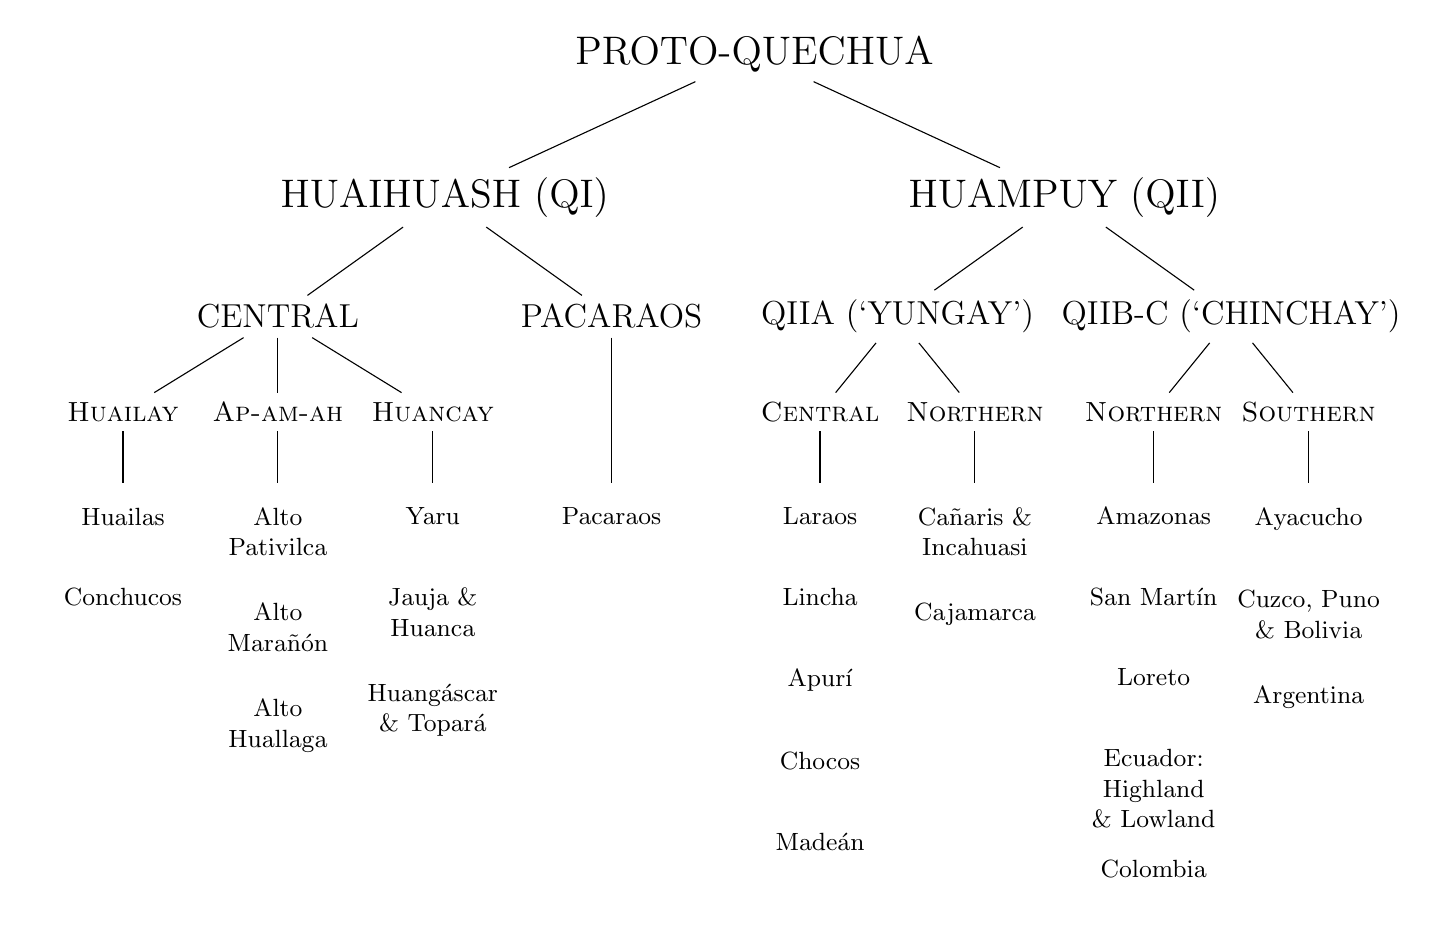
\begin{tikzpicture}[%
treenode/.style = {align=center, inner sep=2ex, text centered},
level 1/.style={sibling distance = 52ex, level distance =12ex,font=\Large}, 
level 2/.style={sibling distance = 28ex, level distance =10ex,font=\large},
level 3/.style={sibling distance = 13ex, level distance =8ex,font=\normalsize\sc},
level 4/.style={treenode,text width=12ex, level distance =6ex,font=\small,below},
level 5/.style={level distance =4ex,edge from parent/.style={draw=none,below}}]
\node[font=\Large] {PROTO-QUECHUA}
  child{node {HUAIHUASH (QI)} 
    child{node {CENTRAL} 
      child{node {Huailay} 
        child{node {Huailas}
          child{node {Conchucos}
          }
        }
      }
      child{node {Ap-am-ah}
        child{node {Alto Pativilca}
          child{node {Alto Marañón} 
            child{node {Alto Huallaga}
            }
          }
        }
      }
      child{node {Huancay} 
        child{node {Yaru}
          child{node {Jauja \&{} Huanca} 
            child{node {Huangáscar \&{} Topará} 
            }
          }
        }
      }
    }
    child{node {PACARAOS}
      child{
        child{node {Pacaraos}
        }
      }
    }
  }
  child{node {HUAMPUY (QII)}
    child{node {QIIA (‘YUNGAY’)} 
      child{node {Central}
        child{node {Laraos}
          child{node {Lincha}
            child{node {Apurí}
              child{node {Chocos}
                child{node {Madeán}
                }
              }
            }
          }
        }
      }
      child{node {Northern}
        child{node {\ili{Cañaris} \&{} Incahuasi}
          child{node {Cajamarca}
          }
        }
      }
    }
    child{node {QIIB-C (‘CHINCHAY’)}
      child{node {Northern}
        child{node {Amazonas}
          child{node {San Martín}
            child{node {Loreto}
              child{node {Ecuador: Highland \&{} Lowland}
                child{node {Colombia}
                }
              }
            }
          }
        }
      }
      child{node {Southern}
        child{node {Ayacucho}
          child{node {\ili{Cuzco}, Puno \&{} Bolivia}
            child{node {Argentina}
            }
          }
        }
      }
    }
  };
\end{tikzpicture}}
\caption{Quechuan languages family tree}\label{Fig1}
% \raggedright
% {\scriptsize Adapted from source:\url{http://lingweb.eva.mpg.de/quechua/Eng/Cpv/Locations.htm#TheTraditionalQuechuaFamilyTree} }
\end{figure}

The Province is located on the border between the two large, contiguous zones where languages belonging to the two great branches of the Quechua language family are spoken: the “Quechua I” (Torero)\index[aut]{Torero, Alfredo} or “Quechua B” (Parker)\index[aut]{Parker, Gary J.} languages are spoken to its north; the “Quechua~II” or “Quechua~A” languages, to its south, as the map in Figure~\ref{Figcomp} shows.

\begin{figure}

\includegraphics[width=0.889\textwidth]{figures/largerregion2.pdf}

\caption{Peruvian languages map}\label{Figcomp} 

\end{figure}

For reasons detailed in \sectref{sec:classification}, the model that divides the Quechuan family tree into two principal branches doesn’t apply very well to Yauyos, as its different dialects manifest different characteristics of both of branches. Yauyos is, of course, not alone in this, not in the least because the division of the languages into two branches was, arguably, based on rather arbitrary criteria in the first place \citep[See in particular][]{Landerman91}.\index[aut]{Landerman, Peter} The significance of Yauyos lies in the fact that it may represent the “missing link” between the two \citep[See in particular][]{Heggarty07}\index[aut]{Heggarty, Paul}. There exist three proposals in the literature --~\citet{Taylor00,Torero74,ethnologue}\index[aut]{Taylor, Gerald}\index[aut]{Torero, Alfredo}\index[aut]{Lewis, M. Paul}~-- with regard to the grouping of the province’s fifteen districts into dialect bundles. \citet[105]{Taylor00}\index[aut]{Taylor, Gerald} counts seven varieties of Yauyos Quechua, dividing these into two groups along a north-south axis. In the north are the dialects of Alis/Tomas, Huancaya/Vitis, and Laraos; in the south, those of Apurí/Chocos/Madeán/Viñac, Azángaro/Huangáscar, Cacra/Hongos, and Lincha/Tana. Taylor classes four of these dialects --~the northern dialects of Alis/Tomas\il{Alis}\il{Tomas} and Huancaya/Vitis\il{Huanca}\il{Vitis} and the southern dialects of Azángaro/Huangáscar\il{Azángaro}\il{Huangáscar} and Cacra/Hongos\il{Cacra}\il{Hongos}~-- as belonging to the \QI{} branch; he classes the remaining three --~Laraos\il{Laraos} in the north as well as Apurí/Cho\-cos/Madeán/Víñac\il{Apurí}\il{Chocos}\il{Madeán}\il{Víñac} and Lincha/Tana\il{Lincha}\il{Tana} in the south~-- as belonging to \QII. \citet{Torero74}\index[aut]{Torero, Alfredo} counted only six dialects, excluding Azángaro/Huangáscar\il{Azángaro}\il{Huangáscar} from the catalogue, classing it independently among the \QI{} dialects along with with Chincha’s Topará\il{Topará}. Ethnologue, like Taylor, includes Azángaro/Huangascar and adds, even, an eighth dialect, that of San Pedro de Huacarpana, spoken on the Chincha side of the Yauyos-Chincha border. Ethnologue further differs from Taylor in putting Apurí in a group by itself; and it differs from both Taylor and Torero in grouping Chocos with Azángaro/Huangáscar. My research supports Taylor’s grouping of Apurí with Madeán and Viñac; it also supports Ethnologue’s inclusion of San Pedro de Huacarpana among the dialects of Yauyos. San Pedro is located immediately to the north-east of Madeán and Azángaro, at less than a days’ walk’s distance. Although formerly counted a part of the Department of Lima and the Province of Yauyos, a redrawing of political boundaries placed San Pedro on the Ica side of the contemporary Ica-Lima border. During the colonial period, the Province of Yauyos was larger and included parts of what are now the Provinces of Chincha and Castrovirreyna (Huancavelica) \citet[1.1.3.2.7]{Landerman91}\index[aut]{Landerman, Peter N.}. Apurí, like its neighbors Viñac and Madeán, uses \phono{-ni} and \phono{-y} to indicate the first-person singular in the verbal and substantive paradigms; they also use \phono{-rqa} and \phono{-sa} to indicate the past tense and perfect. The first pair of characteristics set the Madeán/Viñac and Lincha/Tana dialects apart from the other three; the second pair of characteristics sets Madeán/Viñac apart from Lincha/Tana. Chocos, like its neighbors Huangáscar and Azángaro, uses vowel length to indicate the first-person singular in the verbal and substantive paradigms.

\section{Classification}\label{sec:classification}\index[sub]{classification}
\largerpage %longdistance
Yauyos Quechua was dubbed by Alfredo Torero (\citeyear{Torero74})\index[aut]{Torero, Alfredo} a “supralect” and its most careful student, Gerald Taylor,\index[aut]{Taylor, Gerald} referred to it as a “mixed” language (\citealt[2]{Taylor90}, \citealt[105]{Taylor00}). Indeed, the designation of Yauyos as a language may seem, at first, to be no more than a relic of the first classifications of the Quechuan languages not by strictly linguistic criteria but, rather, by geographic criteria. Yauyos is located on the border between the two large, contiguous zones where the languages of the two different branches of the Quechuan language family are spoken. \QI{} is spoken immediately to the north, in the Department of \ili{Junín} and the north of the Department of Lima; \QII, immediately to the south, in the Departments of Huancavelica and \ili{Ayacucho}. Yauyos manifests characteristics of both branches. Take first-person marking. Three dialects, Azángaro-Chocos\footnote{I am very grateful to Peter Landerman for correcting me with regard to the classification of Chocos, which I had originally misclassified with Madeán and Viñac.}-Huangáscar~(\ACH), Cacra-Hongos (\CH), and San Pedro~(\SP), use the same marking~(vowel length) for the first person in both nominal and verbal paradigms\footnote{Crucially, though, vowel length is not distinctive anywhere else in the grammar or lexicon of these dialects. For example, these dialects use the \QII{}~\phono{-naya},~\phono{-raya}, and~\phono{-paya}, not the \QI{}~\phono{-na:},~\phono{-ra:}, and~\phono{-pa:} to mark the desiderative, passive, and continuative, respectively. And all districts but Cacra use~\phono{tiya-}, not~\phono{ta:-} ‘sit’, again sorting with the \QII{} languages.} and mark the first-person object with~\phono{-ma}. These are the two characteristics that define a Quechuan language as belonging to the \QI{}~(also called Quechua B or~\textit{Huaihuash}) branch. The other two dialects, Apurí-Madeán-Viñac~(\AMV) and Lincha-Tana~(\LT), mark the first person differently in the nominal and verbal paradigms~(with~\phono{-y} and~\phono{-ni}, respectively) and mark first-person object with~\phono{-wa}. These two dialects, then, sort with the \QII{}~(A/\textit{Huampuy})\il{Huampuy} languages. Indeed, the first three are classed as \QI{}~(specifically, Central\textit{-Huancay}) and the other two, \QII{}~(specifically~\textit{Yunagay}-Central) \citep[247]{CerroP87}.\index[aut]{Cerrón-Palomino, Rodolfo M.} Nevertheless, the “\QI” dialects, \ACH, \CH, and \SP, manifest few of the other traits that set the \QI{} languages apart from the \QII{} languages. They do use~\phono{ñuqakuna}\index[sub]{nuqakuna@\phono{ñuqakuna}} in place of \phononb{ñuqayku}\index[sub]{nuqayku@\phono{ñuqayku}} to form the first person plural exclusive as well as~\phono{-pa(:)ku} to indicate the plural. Crucially, however, so do both the “\QII” \SYQ{} dialects.\footnote{The \CH{} dialect is unique in using~\phono{-traw} in alternation with both~\phono{-pi} and~\phono{-pa} for the locative.} And none of the five manifest any other of the principal traits that generally set the \QI{} languages apart from the rest. None use~\phono{-naw} in place of~\phono{-Sina} to form the comparative,~\phono{-piqta} in place of~\phono{-manta} to form the ablative, or~\phono{-naq} in place of~\phono{-shqa} to form the narrative past; and none except for Cacra uses~\phono{-r} (realized \textipa{[l]}) in place of~\phono{-shpa} to form same-subject subordinate clauses. Now, the two “\QII” \SYQ{} dialects manifest several of the traits that set the \QIIC{}~(\textit{Chínchay Meridional}) languages apart from the rest. Like the \QIIC{} languages, the \AMV{} and \LT{} dialects use the diminutive~\phono{-cha}, the emphatic~\phono{-ari}, the assertive~\phono{-puni}, and the alternative conditional~\phono{-chuwan}; the \AMV{} dialect additionally uses the alternative conditional~\phono{-waq.} Crucially, however, the three “\QI” \SYQ{} dialects, too, use three of these:~\phono{-cha},~\phono{-ari} and~\phono{-chuwan}. Further, all five share with \ili{Ayacucho} Q the unique use of the evidential modifier~\phono{-ki}. None of the five manifest any of the other defining traits of the \QIIC{} languages: none uses~\phono{-ku} to indicate the first-person plural exclusive or the third-person plural; nor does any use~\phono{-chka}\footnote{Although all use~\phono{-chka}, unproductively except in \SP, to indicate simultaneous action that persists in time.} to form the progressive or~\phono{-nka} to form the distributive. Further, none suffered the fusion of \textipa{*/tr/} with \textipa{*/ch/} or \textipa{*/sh/} with \textipa{*/s/}. (See \citet[226--248]{CerroP87} on the defining characteristics of the various Quechuan languages)\index[aut]{Cerrón-Palomino, Rodolfo M.} Rather, the dialects of Southern Yauyos are mutually intelligible, and they together share characteristics that set them apart from all the other Quechuan languages. With the single exception that \CH{} uses the accusative form~\phono{-Kta} in place of~\phono{-ta}, all five dialects employ the same case system, which includes the unique ablative form~\phono{-paq} and unique locative \phono{-pi}. All dialects use the progressive form~\phono{-ya};\footnote{One of many attested reductions from *-\phono{yka}: (\phono{-yka:}, \phono{-yka}, \phono{-yga}, \phono{-ycha:}, \phono{-yya:}, \phono{-yya-}, \phono{-ya:}, and \phono{-ya}) \citep[213--219, 260--268, 290]{Hintz}. I am grateful to an anonymous reviewer for pointing this out to me.} all employ the plural~\phono{-kuna} with non-exhaustive meaning; and all employ the same unique system of evidential modification~(see \sectref{ssec:evidmodifi}). 
\largerpage
Further, with a single exception,\footnote{In the \CH{} dialect, as in neighboring \ili{Junín}, the protomorphemes \textipa{*/r/}, \textipa{*/s/}, and \textipa{*/h/} are sometimes realized as \textipa{[l]}, \textipa{[h]}, and \textipa{[sh]}, respectively. I have no explanation for why these alternations occur in some cases but not in others. Indeed, it may be the case that where \CH{} differs from the rest of the dialects in that it employs \textipa{*/sh/}where they employ \textipa{*/h/, it is the former that preserves the original form.}} the five dialects are uniform phonologically, all employing a highly conservative system\footnote{An anonymous reviewer points out that other Quechuan languages, \ili{Corongo} among them, for example, are more conservative than Yauyos with respect to some features, including the preservation of the protoform *ñ in *ñi- ‘say’ and ña:-ña ‘right now’. \ili{Sihuas}, too, preserves elements of proto Quechua not found in Yauyos. In contrast, while Yauyos preserves a few proto-Quechua features not found in either \ili{Corongo} or \ili{Sihuas}, it also manifests others that reflect innovations likely adopted from neighboring QII languages.} that retains all those phonemes hypothesized by Parker and Cerrón-Palomino to have been included in the Proto-Quechua (see \sectref{sec:phoinvmor}). Table~\ref{Tab1}, below, summarizes this information. Please note that the table presents a somewhat idealized portrait and that the characteristics it posits as belonging exclusively to \QII{} may sometimes be found in \QI{} languages as well. Exceptions of which I am aware are signaled in notes to the table.

% TABLE 1
\begin{table}
\renewcommand*{\arraystretch}{0.9}
\centering
\caption{Use of \QI, \QII{} and local structures in the five \SYQ{} dialects}\label{Tab1}
\footnotesize
\begin{tabularx}{0.9\textwidth}{Xccccc}
\lsptoprule
 &\CH &\ACH &\SP &\AMV &\LT\\
\midrule
%
1Singular nominal inflection%
&\Qgreen{\it -:} &\Qgreen{\it -:} &\Qgreen{\it -:} &\Qblue{\it -y} &\Qblue{\it -y} \\
%
1Singular verbal inflection%
&\Qgreen{\it -:} &\Qgreen{\it -:} &\Qgreen{\it -:} &\Qblue{\it -ni} &\Qblue{\it -ni} \\
%
1Singular object inflection%
&\Qgreen{\it -ma} &\Qgreen{\it -ma} &\Qgreen{\it -ma} &\Qblue{\it -wa} &\Qblue{\it -wa} \\
%
1Plural exclusive pronoun~\phono{ñuqakuna}%
&\Qgreen{yes} &\Qgreen{yes} &\Qgreen{yes} &\Qgreen{yes} &\Qgreen{yes} \\
%
Fusion of \textipa{*/ch/} and \textipa{*/tr/}\tabfoot{a}%
&\Qgreen{no} &\Qgreen{no} &\Qgreen{no} &\Qgreen{no} &\Qgreen{no} \\
%
Fusion of \textipa{*/s/} and \textipa{*/sh/}%
&\Qgreen{no} &\Qgreen{no} &\Qgreen{no} &\Qgreen{no} &\Qgreen{no} \\
%
\lsc{s}>\lsc{o} inflection order \lsc{num-o-tns-s}%
& \Qgreen{yes} &\Qgreen{yes} &\Qgreen{yes} &\Qgreen{yes} &\Qgreen{yes} \\
%
Vowel length distinctive elsewhere\tabfoot{b}%
&\Qblue{no} &\Qblue{no} &\Qblue{no} &\Qblue{no} &\Qblue{no} \\
%
Same-subject subordinator~\phono{-shpa}\tabfoot{c}%
&\Qblue{yes} &\Qblue{yes\tabfoot{d}} &\Qblue{yes}&\Qblue{yes} &\Qblue{yes} \\
%
Narrative past inflection~\phono{-sHQa}%
&\Qblue{yes} &\Qblue{yes} &\Qblue{yes} &\Qblue{yes} &\Qblue{yes} \\
%
Comparative~\phono{-hina}%
&\Qblue{yes} &\Qblue{yes} &\Qblue{yes} &\Qblue{yes} &\Qblue{yes} \\
%
Diminutive~\phono{-cha}\tabfoot{e}%
&\Qblue{yes} &\Qblue{yes} &\Qblue{yes} &\Qblue{yes} &\Qblue{yes} \\
%
Emphatic~\phono{-ari}%
&\Qblue{yes} &\Qblue{yes} &\Qblue{yes} &\Qblue{yes} &\Qblue{yes} \\
%
1Plural Altern. Conditional~\phono{-chuwan}%
&\Qblue{yes} &\Qblue{yes} &\Qblue{yes} &\Qblue{yes} &\Qblue{yes} \\
%
2Singular Altern. Conditional~\phono{-waq}%
&\Qgreen{no} &\Qgreen{no} &\Qgreen{no} &\Qblue{yes} &\Qgreen{no} \\
%
Assertive~\phono{-puni}%
&\Qgreen{no} &\Qgreen{no} &\Qgreen{no} &\Qblue{yes} &\Qgreen{no} \\
%
Evidential modifier~\phono{-ki}\tabfoot{f}%
&\Qred{yes} &\Qred{yes} &\Qred{yes} &\Qred{yes} &\Qred{yes} \\
%
Locative~\phono{-pa}%
&\Qred{yes\tabfoot{g}}&\Qred{yes} &\Qred{yes} &\Qred{yes} &\Qred{yes} \\
%
Ablative~\phono{-paq}\tabfoot{h}%
&\Qred{yes} &\Qred{yes} &\Qred{yes} &\Qred{yes} &\Qred{yes} \\
%
Non-exhaustive~\phono{-kuna}%
&\Qred{yes} &\Qred{yes} &\Qred{yes} &\Qred{yes} &\Qred{yes} \\
%
Lateralization of \textipa{*/r/}%
&yes\tabfoot{j} &no &no &no &no\\
\lspbottomrule
\end{tabularx}
\begin{tabularx}{\textwidth}{@{~}r@{~}X@{~}}
\\[-2ex]
Note: &\\
\tabfoottext{a}{An anonymous reviewer points out that this is not exclusively a feature of \QII{} languages in that the fusion of */ch/ and */tr/ is attested in \ili{Huallaga}, a \QI{} variety.}
\tabfoottext{b}{With the exception of~\phono{-pa(:)ku}, where the long vowel distinguishes \lsc{jtacc} from \lsc{ben-refl}.}
\tabfoottext{c}{An anonymous reviewer points out that, although this may originally have been posited to be a defining characteristic of \QII{} languages, it is, in fact, far from such: \phono{-shpa} is common in several QI dialects: in \ili{Ancash}, it attested in \ili{Huaylas}; it is attested, also in Pachitea in \ili{Huanuco}.}
\tabfoottext{d}{Cacra but not Hongos also uses~\phono{-r} (realized \textipa{[l]}).}
\tabfoottext{e}{An anonymous reviewer points out that while diminutive \phono{-cha} is less productive in \QI{} than in \QII, it is still is common throughout \QI, \eg{} Victoria-Vitucha, Cabrito-Kapcha.}
\tabfoottext{f}{Also used in \ili{Ayacucho} (\QII).}
\tabfoottext{g}{Also uses~\phono{-traw} (\QI).}
\tabfoottext{h}{An anonymous reviewer points out that ablative \phono{-paq} is almost certainly derived from */-piq/ / */-pik/ via vowel harmony. The former is attested in \ili{Huaylas} and the latter in \ili{Corongo}. The other \phono{-pi}-initial forms in \QI{} (\phono{-pita}, -\phono{pi:ta}, -\phono{pikta}, -\phono{piqta}, among others) would have developed later via suffix amalgamation, similar to the formation of bipartite \phono{-manta} in \QII{} \citep[see, \eg,][]{hintz2000caracteristicas}.}
\tabfoottext{j}{Also occurs in \ili{Junín} (\QI).}\\[-1ex]
Key: &*:~\QI{} trait; †:~\QII/\QIIC{} trait; ‡:~trait shared by all \SYQ{} dilects not characteristic of either \QI{} or \QII/\QIIC.\\
\end{tabularx}
\end{table}

The case of Azángaro-Chocos-Huangáscar requires particular attention in this context. Torero (\citeyear{Torero68}:~293, \citeyear{Torero74}:~28--29)\index[aut]{Torero, Alfredo} classified Azángaro and Huangáscar as forming an independent group with Topará\il{Topará} (Chavín)\index[sub]{Chavín}, placing it among the \QI{} \phono{Huancay} languages. \citet[236]{CerroP87},\index[aut]{Cerrón-Palomino, Rodolfo M.} following Torero, cites five criteria for grouping Huangáscar with Topará. Both dialects, he writes, use \phono{-pa:ku} and~\phono{-:ri} to indicate the plural; both use~\phono{-shpa} in place of~\phono{-r} to form same-subject subordinate clauses; and both use~\phono{-tamu} to indicate completed action; the two dialects, further, are alike in using unusual locative and ablative case-marking. Only three of these claims are accurate. First, Huangáscar, as \citet{Taylor84}\index[aut]{Taylor, Gerald} already indicated, does not use~\phono{-:ri}. Second, Huangáscar and Topará may indeed both use unusual locative and ablative case marking, but, crucially, they do not use the same unusual case marking: Huangáscar uses~\phono{-pa} to indicate the locative while Topará uses~\phono{-man}; Huangáscar uses~\phono{-paq} to indicate the ablative while Topará uses~\phono{-pa}~(C.-P. himself points out these last two facts). Huangáscar does indeed use~\phono{-shpa} to form subordinate clauses and~\phono{-tamu} to indicate irreversible change. Crucially, however, so do all the dialects of southern Yauyos. In sum, there is no basis for grouping Huangáscar with Topará and not with the other dialects of \SYQ. Torero’s data were never corroborated; indeed, the findings of Taylor and Landerman, the scholars who have most thoroughly studied Yauyos before now,\footnote{An anonymous reviewer points out that Martha Hardman, Steve Echerd, Rick Floyd, Conrad Phelps --~in addition to several students from Universidad San Marcos~-- have given Yauyos extensive attention, although they may not have added to the storehouse of data on the language.} contradict those of Torero.

\SYQ{} is not a jumble of dialects that, were it not for geographical accident, would not be classed together; it is, rather, a unique, largely uniform language. Although I myself do not believe that the current paradigm can be maintained, I have tried to present the data in a way that remains as neutral as possible with regard to the question of how the internal diversity within the Quechuan language family is best characterized, and, in particular, with regard to the question of whether or not the various Quechuan languages are helpfully construed as belonging to one or the other of two branches of a family tree \citep[See in particular][]{Adelaar08}.\index[aut]{Adelaar, Willem F. H.} I leave it to other scholars to interpret the data as they see fit. That said, as long as it is maintained, the current paradigm should be revised to more accurately reflect the relationships of \SYQ{} with/to the languages currently named on the Quechuan family tree as it is currently drawn. That tree groups nine of the eleven districts of southern Yauyos into five sets, assigning each of these sets the status of an independent language. Moreover, two of these sets are actually singletons, as Chocos is listed independent of \mbox{(Azángaro-)}Huangáscar, to which it is identical, and Apurí is listed independent of Madeán(-Viñac), to which it is identical. (Cacra-Hongos, the set that would deserve independent placement, if any did, appears nowhere at all). The fact that all these “languages” are completely mutually intelligible does not justify this. It further seems unjustified to place the Quechua of single villages on the level of that of whole nations --~Bolivia and Ecuador. I suggest, therefore, that Chocos be joined with \mbox{(Azángaro-)}Huangáscar, and Apurí with Madeán(-Viñac). The first of these new triplets, Azángaro-Chocos-Hunagáscar, should be mutated to join the other “languages” of southern Yauyos, under the category \textit{Central Yungay}. The four sets should, further, be collapsed and the resulting set called \textit{Southern Yauyos}. The revised (pruned) tree would then be as in Figure~\ref{Fig1rev}. In the event that it be necessary to honor the internal diversity that would be obscured by this move, note may simply be made to the fact that this “new” language counts multiple dialects. In this case, Cacra-Hongos and San Pedro de Huacarpana would have to be listed among these.\footnote{I regret having to list Laraos independently here, as I believe it is possible to make a convincing argument for its inclusion as a dialect of Southern Yauyos. Nothing in this volume, however, directly speaks to that question. I plan to address it explicitly in a future paper.}

% REVISED TREE
% http://lingweb.eva.mpg.de/quechua/Eng/Cpv/Locations.htm#TheTraditionalQuechuaFamilyTree
% Adapted from
\begin{figure}[!ht]

\il{Proto-Quechua}\il{Huaihuash}\il{Huailay}\il{Huailas}\il{Conchucos}\il{Ap-am-ah}\il{Alto Pativilca}\il{Alto Marañón}\il{Alto Huallaga}\il{Yaru}\il{Jauja}\il{Huanca}\il{Pacaraos}\il{Huampuy}\il{Yungay}\il{Laraos}\il{Cañaris}\il{Incahuasi}\il{Cajamarca}\il{Chinchay}\il{Amazonas}\il{San Martín Quechua}\il{Loreto}\il{Ecuadorian Quechua}\il{Colombian Quechua}\il{Ayacucho}\il{Cuzco}\il{Puno}\il{Bolivian Quechua}\il{Argentinan Quechua}
\resizebox{\textwidth}{!}{%
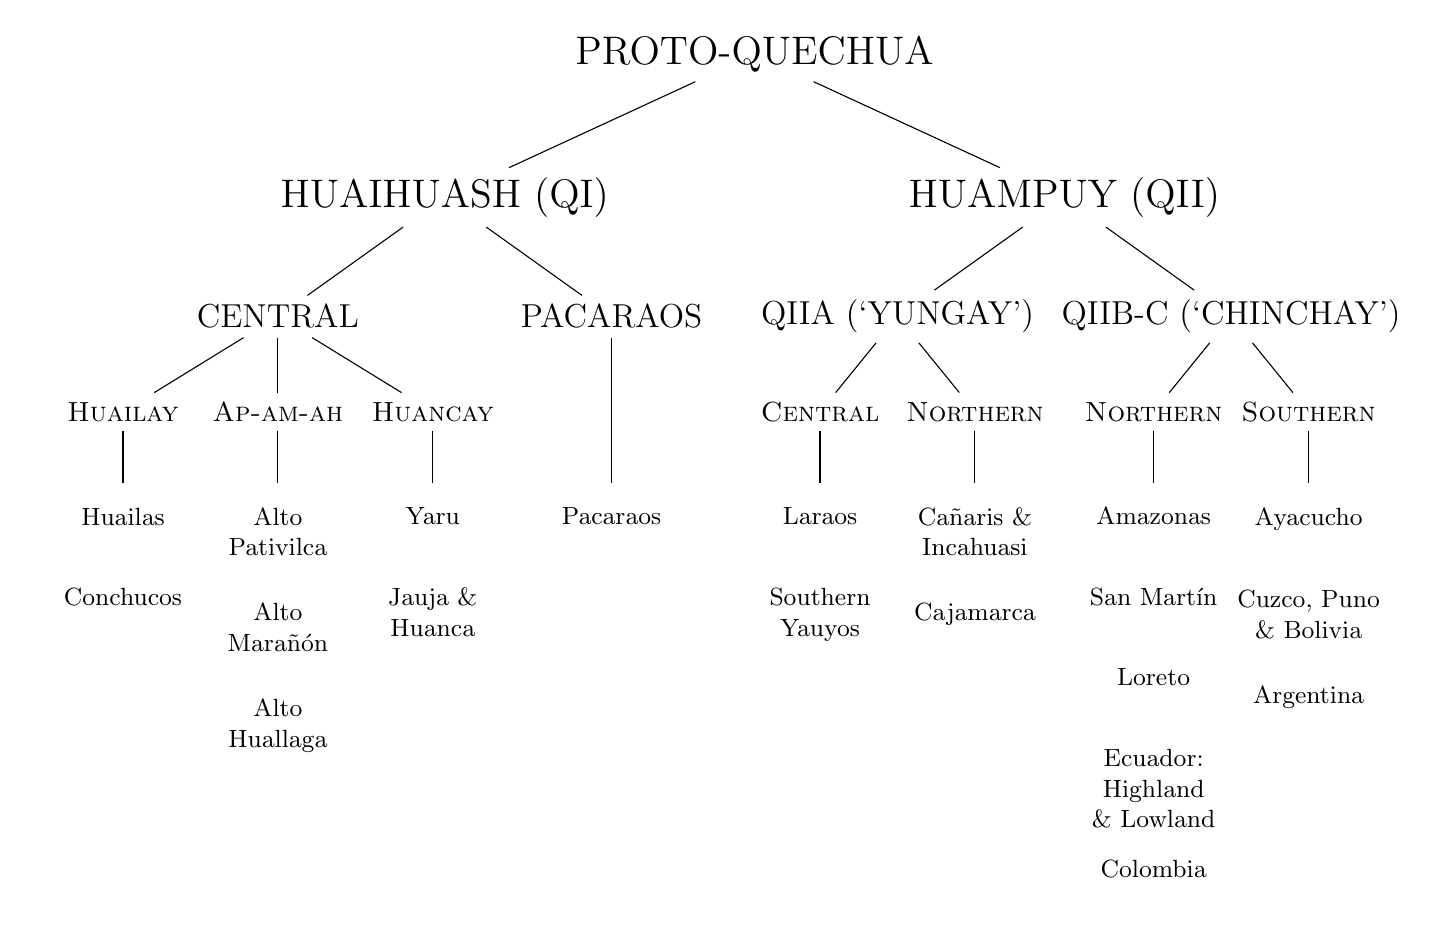
\begin{tikzpicture}[%
treenode/.style = {align=center,inner sep=2ex,text centered},
level 1/.style={sibling distance=52ex,level distance=12ex,font=\Large}, 
level 2/.style={sibling distance=28ex,level distance=10ex,font=\large},
level 3/.style={sibling distance=13ex,level distance=8ex,font=\normalsize\sc},
level 4/.style={treenode,text width=12ex,level distance=6ex,font=\small,below},
level 5/.style={level distance=4ex,edge from parent/.style={draw=none,below}}]
\node[font=\Large] {PROTO-QUECHUA}
  child{node {HUAIHUASH (QI)} 
    child{node {CENTRAL} 
      child{node {Huailay} 
        child{node {Huailas}
          child{node {Conchucos}
          }
        }
      }
      child{node {Ap-am-ah}
        child{node {Alto Pativilca}
          child{node {Alto Marañón} 
            child{node {Alto Huallaga}
            }
          }
        }
      }
      child{node {Huancay} 
        child{node {Yaru}
          child{node {Jauja \&{} Huanca} 
          }
        }
      }
    }
    child{node {PACARAOS}
      child{
        child{node {Pacaraos}
        }
 	  }
    }
  }
  child{node {HUAMPUY (QII)}
    child{node {QIIA (‘YUNGAY’)} 
      child{node {Central}
        child{node {Laraos}
          child{node {Southern Yauyos}
          }
        }
      }
      child{node {Northern}
        child{node {\ili{Cañaris} \&{} Incahuasi}
          child{node {Cajamarca}
          }
        }
      }
    }
    child{node {QIIB-C (‘CHINCHAY’)}
      child{node {Northern}
        child{node {Amazonas}
          child{node {San Martín}
            child{node {Loreto}
              child{node {Ecuador: Highland \&{} Lowland}
                child{node {Colombia}
                }
              }
            }
          }
        }
      }
      child{node {Southern}
        child{node {Ayacucho}
          child{node {\ili{Cuzco}, Puno \&{} Bolivia}
            child{node {Argentina}
            }
          }
        }
      }
    }
  };
\end{tikzpicture}}

\caption{Quechuan languages family tree revised}\label{Fig1rev}
\raggedright
{\scriptsize Adapted from source: \url{http://lingweb.eva.mpg.de/quechua/Eng/Cpv/Locations.htm#TheTraditionalQuechuaFamilyTree}}
\end{figure}

\section{Presentation}\label{sec:presentation}
To facilitate comparison with other Quechuan languages, the presentation here follows the structure of the six Quechua grammars published by the Peruvian government in~1976. Readers familiar with those grammars will note the obvious debt this one owes to those: it follows not just their format, but also, in large part, their analysis. The six~1976 grammars cover the Quechuas of \ili{Ancash}, \ili{Ayacucho}, \ili{Cajamarca}, \ili{Cuzco}, \ili{Huanca} and \il{San Martín Quechua}San Martín. \citep{Parker76gram,Soto76a,Quesada76,Cusihuaman76,CerroP76a,Coombs76}.\index[aut]{Parker, Gary J.}\index[aut]{Soto Ruiz, Clodoaldo}\index[aut]{Quesada Castillo, Félix}\index[aut]{Cusihuamán Gutiérrez, Antonio}\index[aut]{Cerrón-Palomino, Rodolfo M.}\index[aut]{Coombs, David}\index[aut]{Coombs, Heidi}\index[aut]{Weber, Robert} Other published grammars of Quechuan languages include \citet{Herrero78}\index[aut]{Herrero, Joaquín}\index[aut]{Sánchez de Lozada, Federico} on \ili{Bolivian Quechua}; \citet{Catta94}\index[aut]{Catta, Javier} on \ili{Ecuadorian Quechua}; \citet{Taylor94a}\index[aut]{Taylor, Gerald} on \ili{Ferreñafe}; \citet{Weber89}\index[aut]{Weber, David} on \ili{Huallaga}~(\ili{Huanuco});\footnote{Thanks to an anonymous reviewer for pointing this out. \citet{Hintz} supplies a grammar of aspect and related categories in Quechua, especially South \ili{Conchucos} Quechua (\ili{Ancash}).} \citet{Cole82}\index[aut]{Cole, Peter} on \ili{Imbabura}; \citet{Adelaar77}\index[aut]{Adelaar, Willem F. H.} description of \ili{Tarma} Quechua and his (\citeyear{Adelaar86}) morphology of \ili{Pacaraos}; 
as well as the surveys and compilations of \citet{CerroP87,CerroP90}\index[aut]{Cerrón-Palomino, Rodolfo M.}\index[aut]{Solís-Fonesca, Gustavo}, and \citet{Cole94}\index[aut]{Cole, Peter}\index[aut]{Hermon, Gabriella}\index[aut]{Martín, Mario D.}.

Words and phrases appearing in italics --~\phono{like this}~-- are in Quechua. English and Spanish interpretations appear in single quotation marks --~‘like this’. Interpretations are sometimes given in Spanish --~the language I used with my consultants\footnote{Indeed, all English glosses are my translations from the Spanish glosses my consultants originally supplied. In most cases, the Spanish translations reflected the syntax and semantics of the original Quechua. I sacrificed this in preparing the the English glosses that appear here. I made this choice because the more literal glosses are standard in Andean Spanish --~in structures like the possessive ‘su n de a’ (‘his \lsc{n} of a’)~-- they would not be standard in any English dialect of which I am aware.} --~as well as English. Transformations (illustrations of changes indicated as a result of morphological processes referenced) are indicated with arrows --~\textit{like}~→~\textit{like\_this}. Quechua words are broken into component morphemes, like this: \phono{warmi-\pb{kuna}}. It is the morpheme relevant to the topic in focus that is in bold. 

Each section and major subsection begins with an account of the topic under consideration. Terminal subsections supply more extended discussion and further examples, generally about 10, often as many as 30 or even 40. All examples except those indicated with a dagger are taken from the corpus of recordings collected during the course of the documentation of the language. Those with a dagger were elicited. Transcriptions can be checked against the original recordings by downloading the compilation of recordings archived with the corpus, typing a couple of words from either the example or its gloss into the search bar and following the recording title and time signature back to the original recording. I am also happy to supply this information. Source titles refer to \textrm{.eaf} files archived with DoBeS\index[sub]{DoBeS} and AILLA\index[sub]{AILLA}. File names include three elements: the place in which the recording was made, the initials of the principal participant, and a word or two recalling the principal topic(s). For example, the file \textrm{Vinac\_JC\_Cure} was made in Viñac, has for its principal participant Jesús Centeno and for its principal topic a curing ceremony. Because of restrictions on file names, no accents are used. So, Az\pb{á}ngaro is rendered “Az\pb{a}ngaro” and so on.

Glosses were prepared in accord with the Leipzig glossing rules. For reasons of space, two deviations from the standard abbreviations were made: “proximal demonstrative” is not rendered “\lsc{dem.prox}” but “\lsc{dem.p}”; and “distal demonstrative” is not rendered “\lsc{dem.dist}” but “\lsc{dem.d}”. Gloss codes are listed with the notational conventions at page~\pageref{ch:notconv}, in the section with that name.

\section{Fieldwork} \label{sec:fieldwork}
The fieldwork upon which this document is based was conducted in June and July of~2010; January through April~2011; August through December~2011; April through September~2012; and for a total of~10 months between October~2012 and July~2014. The second of these trips was funded by a faculty development grant from San José State University; the third through sixth, by two National Endowment for the Humanities-National Science Foundation Documenting Endangered Languages fellowships~(FN-50099-11 and FN-50109-12).

The corpus counts 206 distinct audio and audio-video recordings. The recordings\index[sub]{recordings}, totaling over~71 hours, were made in the seven districts of Southern Yauyos --~Apurí, Azángaro, Cacra, Chocos, Hongos, Hu\-angáscar, Lincha, Madeán, and Viñac~-- as well as in the district of San Pedro de Huacarpana in Chincha. Recordings include stories, songs, riddles, spontaneous dialogue, personal narrative, and descriptions of traditional activities, crafts and healing practices. Over~28 hours of recordings were transcribed, translated and glossed. The recordings as well as the ELAN time-aligned transcriptions and accompanying videos are archived both at The DoBeS project\index[sub]{DoBeS}, housed at the Max Planck Institute in Nijmegen, The Netherlands, and at the Archive of the Indigenous Languages of Latin America at the University of Texas, Austin, USA. All materials can be accessed via those institutions’ websites, \url{http://www.mpi.nl/DOBES/} and \url{http://www.ailla.utexas.org/}. The more popular video recordings --~many transcribed~-- can also be easily accessed via \url{endangeredlanguages.com}. All examples that follow except those noted † were taken from this corpus. It is my hope that these examples will give the reader a sense of the life that supported and was supported by the language. 

Unicode was used for character encoding; audio and video recordings were saved in the standard formats --~PCM \textrm{wav}~44.1/32~bits, \textrm{.mpg}, and \textrm{.mpeg}; unstructured texts were saved as plain text; structured texts have XML-based underlying schemas. Recording equipment includes a Marantz PMD~660 solid state digital audio recorder~(pre-January~2013 recordings); a Roland~R-26 solid state audio recorder; an AudioTechnica~831b cardioid condenser microphone~(pre-May~2012 recordings); a Sennheiser MKH~8060 cardioid condenser microphone; and a Canon Vixia HF S100 HD flash memory camcorder. Transcriptions, translations and glosses were prepared with ELAN; Audacity was used for editing audio recordings; iMovie for video recordings. All work was done on a MacBook Pro~(pre-July~2011 recordings) or MacBook Air~(post-July~2011 recordings). 

Exactly one hundred participants contributed recordings: AA, DO, Pedro Carrún (Apurí);
Victoria Díaz, Gabino Huari, Ernestina Huari, Efrén Yauri (Madeán);
Isabel Chávez (Tayamarka);
Dona Alvarado, Eudosia Alvarado, Pripodina Auris, Jesus Centeno, Meli Chávez, Delfina Chullukuy, Martina Guerra, Victoria Guerra, Carmen Huari, Aleka Madueño, Acención Madueño, Melania Madueño, Hilda Quispe, Angélica Romero, Saturnina Utcañe (Viñac);Margarita Madueño (Casa Blanca); Floriana Centeno, Emilia Guerra (Esmeralda); Juana Huari, Leonarda Huari, Neri Huari, Corsinia Javier, Cecilia Quispe (Florida); AB (Ortigal); Octavia Arco, Bautista Cárdenas (Llanka); Octavio Sulluchuco (Qanta); Cecilia Guerra, Emiliano Rojas (Qunyari); María Guerra, Teresa Guerra, Alejandra Quispe (Shut\-co); Alejandrina Centeno, Macedonia Centeno, Soylita Chullunkuy, Hida Evangelista, Soylita Huari (Tambopata); Urbana Yauri (Yuracsayhua); Anselma Caja, Filipa Postillón (Azángaro); Genoveva Rodríguez, Lucía Rodríguez (Colca); Fortunato Gutiérrez, Isak Gutiérrez (Marcalla); Alcibiada Rodríguez (Puka Rumi); Victorina Aguado, Senovia Gutiérrez (Villaflor); Honorato B., Bonifacia de la Cruz, Julia Mayta (Chocos); Benedicta Lázaro, CW,  Luisa Gutiérez, PP, Victoria Quispe, Teódolo Rodríguez, Natividad Saldaña (Huangáscar); Grutilda Saldaño; Eudisia Vicente (Tapalla); Iris Barrosa, Maximina Barrosa, Regina Huamán (Cacra); Archi V., Eduardo Centeno, Dina Huamán, Leona Huamán, SA, Sabina Huamán, Senaida Oré, Hipólita Santos, Maximina Tupac, Erlinda Vicente (Hongos); Ninfa Flores, Anselma Vicente, Sofía Vicente (Lincha); Amador Flores, Ga\-bi\-na Flores, Lucio Flores, Dina Lázaro, Elisa Mancha, Isabel Mancha (Tana); Santa Ayllu, Edwin Fuentes, Neli Fuentes, Elvira Huamán, Sofía Huamán, Lucía Martinez, RF, Rosa O., Maximina Paloma, Juan Páucar (Liscay).

\newpage 
For help with transcription and the lexicon, unending thanks to \foreignlanguage{spanish}{Benedicta Lázaro} and Martina \ Reynoso~(\ACH); Mila Chávez, Delfina Chullunkuy, \foreignlanguage{spanish}{Esther Madueño}, Hilda Quispe, and Celia Rojas~(\AMV); Iris Barrosa, Gloria Cuevas, Senaida Oré, Hipólita Santos, and Erlinda Vicente,~(\CH); Ninfa Flores and Sofía Vicente (\LT); and Santa Ayllu, Elvira Huamán, Sofía Huamán, and Maximina Paloma~(\SP).

\section{A note to Quechuanists and typologists}\label{sec:notetoquechuanists} 
Those already familiar with Quechuan languages will likely be interested in the tables and sections listed in Tables~\ref{tab:tabinterestq} and~\ref{tab:secinterestq} immediately below. These indicate differences between Southern Yauyos Quechua and other Quechuan languages as well as differences among the various dialects of \SYQ. The footnotes appearing in these sections may be of interest as well. Those familiar with the literature on Quechuan languages will immediately recognize the presentation and analysis here as very much derivative of much previous work on those languages.\\

% MINI TOC
\noindent
\begin{table}
\centering
\caption{Tables of more interest to Quechuanists}\label{tab:tabinterestq}
\noindent
\begin{tabularx}{\textwidth}{@{~}X}
\lsptoprule
\end{tabularx}
% chapter 1
\minitoctab{Tab1}{Use of \QI, \QII{} and local structures in the five \SYQ{} dialects}
% chapter 2
\minitoctab{Tab5}{Vowel inventory}
\minitoctab{Tab6}{Consonant inventory}
% chapter 4
\minitoctab{Tab11}{Case suffixes with examples}
\minitoctab{Tab12}{Verbal inflectional suffixes with different realizations in \SYQ{} dialects}
\minitoctab{Tab13a}{Verbal inflection paradigm}
\minitoctab{Tab13b}{Verbal inflection paradigm -- subject-object suffixes}
\minitoctab{Tab15}{Actor-object inflectional suffixes}
\minitoctab{Tab27}{“Modal” (verb-verb derivational) suffixes, with examples}
% chapter 6
\minitoctab{Tab30}{Enclitics, with examples}
\minitoctab{Tab31}{Evidential schema: “evidence from” by “evidence for”}
\begin{tabularx}{\textwidth}{@{~}X}
\lspbottomrule
\end{tabularx}
\end{table}

% MINI TOC
\noindent
\begin{table}
\centering
\caption{Sections of more interest to Quechuanists}\label{tab:secinterestq}
\noindent
\begin{tabularx}{\textwidth}{@{~}X}
\lsptoprule
\end{tabularx}
% Chapter 1
%\minitoc{}{}
\minitoc{sec:classification}{Classification}
\minitoc{sec:brin}{Broader interest}
\minitoc{sec:endangerment}{Endangerment}
% Chapter 2
\minitoc{sec:phoinvmor}{Phonemic inventory}
% Chapter 3
\minitoc{ssec:ppnqp}{Personal pronouns \phono{ñuqa}, \phono{qam}, \phono{pay}}
\minitoc{ssec:alloP}{Allocation}
\minitoc{ssec:case}{Case}
\minitoc{ssec:genlocpa12}{Genitive, locative \phono{-pa\tss{1}}, \phono{-pa\tss{2}}}
\minitoc{ssec:ablbenpur}{Ablative, benefactive, purposive \phono{-paq}}
\minitoc{ssec:genlocpi}{Genitive, locative \phono{-pi}}
\minitoc{sssc:inf}{Infinitive \phono{-y}}
\minitoc{ssec:accomp}{Accompaniment \phono{-nti(n)}, \phono{-kuna}}
% Chapter 4
\minitoc{sec:onomatopoeicverbs}{Onomatopoetic verbs}
\minitoc{ssec:subjallo}{Subject and allocation suffixes}
\minitoc{ssec:actorobjref}{Actor and object reference}
\minitoc{par:simplepast}{Simple past \phono{-RQa}}
\minitoc{par:QSPT}{Quotative simple past tense \phono{-sHQa}}
\minitoc{ssec:regcond}{Regular conditional \phono{-man}}
\minitoc{ssec:modality}{Excursis: Modality}
\minitoc{ssec:altcond}{Alternative conditional \phono{-waq} and \phono{-chuwan}}
\minitoc{ssec:progressive}{Progressive \phono{-ya}}
\minitoc{ssec:durative}{Durative, simultaneous \phono{-chka}}
\minitoc{ssec:perfective}{Perfective \phono{-ku}}
\minitoc{par:freqkatra}{Frequentive \phono{-katra}}
\minitoc{par:urgpers}{Urgency/personal interest \phono{-RU}}
% chapter 5
\minitoc{sec:interjections}{Interjections}
% chapter 6
\minitoc{ssec:evidence}{Evidence (entire subsection)}
\begin{tabularx}{\textwidth}{@{~}X}
\lspbottomrule
\end{tabularx}
\end{table}
\clearpage 

\section{Broader interest}\label{sec:brin}
Yauyos should be of particular interest to semanticists as well as to students of language contact. Semanticists may find the language’s unusual evidential system of interest, while students of language contact may want to look for evidence of contact between the districts where Yauyos is spoken --~that of Cacra-Hongos in particular~-- with the three \ili{Aymara}-speaking districts in the same region of the province.

\subsection{Semantics -- evidentials}
For typologists and semanticists, Yauyos’ evidential system should be of interest. Evidentials, broadly speaking, are generally said to indicate the type of the speaker’s source of information. \SYQ, like most other Quechuan languages, employs a three-term system,\footnote{An anonymous reviewer points out that South \ili{Conchucos} has a 5-choice evidential system, and \ili{Sihuas} a 6-choice system \citep{Hintz14}\index[aut]{Hintz, Daniel}, while \ili{Huallaga} has a 4-choice system \citep{Weber89}.\index[aut]{Weber, David John}} indicating direct, reportative, and inferred evidence (\ie~the speaker has personal-experience evidence for~\phono{P}, the speaker has non-personal-experience evidence for~\phono{P}, or the speaker infers~\phono{P} based on either personal- or non-personal-experience evidence). In \SYQ, the three evidentials are realized~\phono{-mI}, \phono{-shI}, and~\phono{-trI} (See \citet{Floyd99} on Wanka Quechua; \citet{Faller03} on \ili{Cuzco} Quechua).\index[aut]{Floyd, Rick}\index[aut]{Faller, Martina} The evidential system of \SYQ{} is of particular interest because it employs a second three-term system of evidential modifiers. The evidential system of \SYQ{} thus counts nine members:~\phono{-mI},~\phono{-mik}, and~\phono{-miki};~\phono{-shI},~\phono{-shik}, and~\phono{-shiki}; and~\phono{-trI},~\phono{-trik}, and~\phono{-triki}. The~\phono{-I}~\phono{-ik}, and~\phono{-iki} forms are not allomorphs: they receive different interpretations. \sectref{ssec:evidence} describes this system in detail. (For further formal analysis, see \citealt{Shimelman12} and \citealt{Shimelman14}\index[aut]{Shimelman, Aviva}).

\subsection{Language contact -- \ili{Aymara}}
For students of language contact, it is the contact of Yauyos with Aymara\il{Aymara} that should be of particular interest.\footnote{Contact of Quechuan languages with Spanish, of course, is of interest here, as it is in all Quechuan languages.} The northern branch of the Aymara family is situated entirely in the province of Yauyos \citep[173]{Adelaar04}\index[aut]{Adelaar, Willem F. H.}\index[aut]{Muysken, Pieter C.}: the Aymaran languages \ili{Kawki} and \ili{Jaqaru} are spoken in the central Yauyos municipalities of Cachuy\index[sub]{Cachuy}, Aysa\index[sub]{Aysa} and Tupe\index[sub]{Tupe}. There are, further, reports dating from the beginning of the~20th century of other Aymaran-speaking communities in the province~(174).\footnote{On Aymara and the relationship of Quechua and Aymara see, among others, Adelaar with Muysken~(\citeyear{Adelaar04}:~259--317)\index[aut]{Adelaar, Willem F. H.}\index[aut]{Muysken, Pieter C.} and \citet{CerroP94,CerroP00}.\index[aut]{Cerrón-Palomino, Rodolfo M.} On \ili{Jaqaru}, see, among others, \citet{Hardman66,Hardman83,Hardman00}.\index[aut]{Hardman, Martha J.}} I was unable to find evidence of any unusual lexical borrowing in Yauyos, \ie,~of words --~like (\phono{pampa-} ‘bury’)~-- not also attested in other Quechuan languages. That said, the lexicon I assembled includes only 2000 words, in large part because the vocabulary of the language has been much-reduced, as is to be expected, given that such reduction is one of the symptoms of extreme language endangerment. Those more familiar with the Aymaran languages may, however, still be able to find evidence of calquing or structural influence.


